\subsection{Datum}
\subsubsection{Gedrag}
Na een reset of \'e\'en keer per dag om 12 uur middernacht zal het datum component de data voor de nieuwe datum verzenden naar de zend buffer. De inkomende data is in het binary coded decimal (bcd) formaat. Eerst zal hij de dag van de week doorgeven, daarna de dag van de maand, de maand en daaropvolgend het jaartal. Dat allemaal sequentieel, getriggert op de neergaande klokflank van de ready$\_$buf. 

\begin{figure}
  \centering
     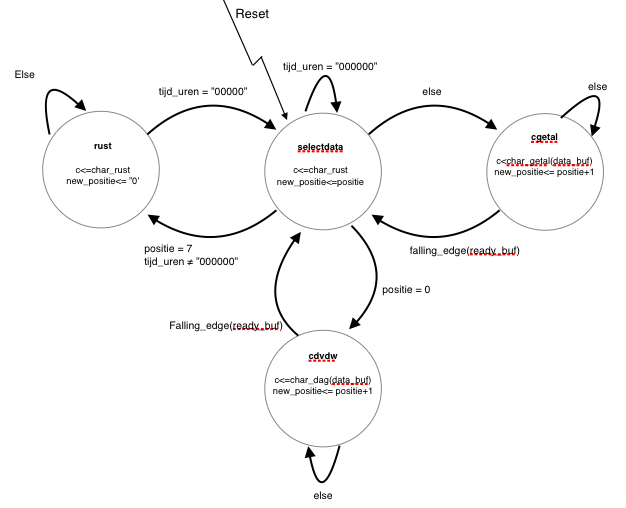
\includegraphics[angle = 0, scale= 0.75{verslag_schemas/datum_entity.png}
       \caption{Entity datum}
\label{fig:simlayout}
\end{figure}


\subsubsection{Functionaliteit}
Het component werkt met een finite state machine (FSM) waarin de characters worden klaargezet en een counter genaamd positie wordt aangestuurd met daarnaast een apart process om de juiste input te bepalen afhankelijk van de counter. \\
Na de reset zal de FSM in de selectdata state starten en positie op 0 worden gezet. 
In het aparte process zal de de data$\_$buf worden gekoppeld aan de input die hoort bij positie=0 en zal de x en y bepaald worden. 
 In selectdata zal  afhankelijk van de counter (in dit geval 0) worden bepaald of de dag van de week of de getallen van de datum moet worden geschreven. Bij positie=0 zal het karakter van de dag van de week (in state cdvdw) worden klaargezet. Het karakter wordt bepaald door de waarde die op de data$\_$buf staat. Op de neergaande klokflank van het ready$\_$buf signaal zal de FSM terug gaan naar de state selectdata en zal er bij positie 1 worden opgeteld. Daardoor zal hierna het eerste getal van de datum worden geschreven. Dit zal zich herhalen tot positie =7, daarna zal hij naar de rust stand gaan en is de datum geschreven. \\
 Als het middernacht is, dus tijd$\_$uren = '00000', zal er ook een nieuwe datum worden klaargezet. Zodra de positie 7 is zal de machine in state selectdata blijven hangen totdat de tijd$\_$uren ongelijk is aan "00000". Dit om te voorkomen dat het component een uur lang onnodig data blijft verzenden. 


\subsubsection{FSM}
\begin{figure}
  \centering
     \includegraphics[angle = 0, scale= 0.6]{verslag_schemas/datum_fsm.png}
       \caption{FSM Datum}
\label{fig:simlayout}
\end{figure}

\subsubsection{VHDL code}
Zie \ref{code:ent_datum} voor de entity code. \\
Zie \ref{code:beh_datum} voor de behavioural code.
Zie \ref{code:datum_tb} voor de testbench die is gebruikt.
\subsubsection{Simulaties}
Zie \ref{ap:sim_datum_behavioural} voor de simulatie van de behavioural code. \\
Zie \ref{ap:sim_datum_circuit} voor de simulatie van het gesynthetiseerde circuit. 
De simulaties zijn uitgevoerd met een clock van 2000ns.  Er is getest tot 300k ns, zie de testbench in \ref{code:datum_tb} voor meer informatie.

\subsubsection{Resultaten}
Uit de simulaties is gebleken dat het circuit doet waarvoor het is ontworpen.
